\documentclass{beamer}

\RequirePackage { geometry }
\RequirePackage { setspace }
\RequirePackage { microtype }
\RequirePackage { enumitem }
\RequirePackage [ spanish ] { babel }
\RequirePackage { csquotes }
\RequirePackage { biblatex }
\RequirePackage { xcolor }
\RequirePackage { hyperref }
\RequirePackage { graphicx }
\RequirePackage { mathtools, amsthm, amsfonts }
\RequirePackage { dirtytalk }
\RequirePackage [ spanish ] { cleveref }
\RequirePackage { epigraph }

\ExplSyntaxOn
\makeatletter

% Cref
\crefname{section}{\S}{\S}

% Set page margins
\geometry
    {
        includehead,
        paper = letterpaper,
        left = 3cm,
        right = 2cm,
        bottom = 2cm,
        top = 2cm,
        marginparsep = 10pt,
        marginparwidth = 2cm,
    }

% Set fonts
\usepackage[lf]{Baskervaldx} % lining figures
\usepackage[bigdelims,vvarbb,baskervaldx]{newtxmath} % math italic letters from Nimbus Roman
\usepackage[cal=boondoxo]{mathalfa} % mathcal from STIX, unslanted a bit
\usepackage[scale=.9]{courierten}
\newcommand{\titlefont}{\bfseries}

% Set basic spacing
\setlength { \parindent } { 8.46pt }
\setlength { \parskip } { 6pt }
\onehalfspacing

% Headers and footer
\pagestyle{headings}
\gdef\@oddhead{\hfil\thepage}

% Bibliography
\addbibresource{references.bib}

% Hyperref
\hypersetup
    {
        colorlinks = true,
        allcolors = black,
    }

% Theorems
\newtheoremstyle{defi}% hnamei
    {.5\baselineskip}% hSpace abovei
    {.5\baselineskip}% hSpace belowi
    {}% hBody fonti
    {}% hIndent amounti
    {\scshape}%\addfontfeatures{LetterSpace=5}}% hTheorem head fonti
    {.}% hPunctuation after theorem headi
    {.5em}% hSpace after theorem headi
    {}% hTheorem head spec (can be left empty, meaning ‘normal’)i
\theoremstyle{defi}
\newtheorem{defi}{Definición}[chapter]

% Sectioning commands
\usepackage[explicit]{titlesec}
\titleformat
    {\chapter}
    [display]
    {\titlefont}
    {
        \centering
        \fontsize{14}{14}\selectfont
        \UpperCase{Capítulo}~\thechapter\\[10pt]
        \fontsize{12}{12}\selectfont
        \UpperCase{#1}
    }
    {0ex}
    {\centering}
\titleformat{name=\chapter, numberless}
    [block]
    {\titlefont}
    {\fontsize{14}{14}\selectfont\UpperCase{#1}}
    {0ex}
    {\centering}
\titleformat
    {\section}
    {\titlefont}
    {\thesection\fontsize{12}{12}\selectfont\ #1}
    {0ex}
    {}
\titleformat{name=\section, numberless}
    [block]
    {\titlefont}
    {\fontsize{12}{12}\selectfont #1}
    {0ex}
    {}

% USB logo
\cs_set_eq:NN \latex_centering:D \centering

\cs_new:Npn \th_print_logo_head:n #1
    {
        \group_begin:
            \latex_centering:D
            \includegraphics[scale=.3]{resources/usblogo} \\
            { \titlefont \UpperCase{#1} }
            \tex_par:D
        \group_end:
    }

\NewDocumentCommand{ \UpperCase }{ m }
    {
        \group_begin:
        %\addfontfeatures{LetterSpace=10}
        \text_uppercase:n { #1 }
        \group_end:
    }

\NewDocumentCommand{ \UppercaseBold }{ m }
    {
        { \titlefont\UpperCase{#1} }
    }

\NewDocumentCommand{ \PrintUsbLogo }{ m }
    {
        \th_print_logo_head:n { #1 }
    }

\NewDocumentCommand{ \ToC }{}
    {
        \chapter*{Índice~General}
        \@starttoc{toc}
    }

% Notes
\reversemarginpar
\NewDocumentCommand{ \note }{ m }
{
    \marginpar
    {
        \color{blue}
        \raggedleft
        \sffamily
        \scriptsize
        #1
        \PackageWarning{Notes}{Revisar~nota}
    }
}

% Wrapping
\newlength{\wrapwd}
\NewDocumentCommand { \wrapto } { o o m }
{
    \IfNoValueTF { #1 }
        { \setlength{\wrapwd}{.6\linewidth} }
        { \setlength{\wrapwd}{#1} }
    \IfNoValueTF { #2 }
        { \let\wrapal\raggedright }
        { \let\wrapal#2 }
    \begin{minipage}{\wrapwd}
        \wrapal
        #3
    \end{minipage}
}

% Conditionals
\newif { \ifcaratula }
\newif { \ifpaginatitulo }
\newif { \ifresumen }
\newif { \ifdedicatoria }
\newif { \ifagradecimientos }
\newif { \iftoc }
\newif { \ifsimbolos }
\newif { \ifabreviaturas }
\newif { \ifintro }
\newif { \ifbasicos }
\newif { \ifreferencias }

% macros
\newcommand { \MainTitle }
    {
        Estudio~comparativo~de~tres~demostraciones~
        del~teorema~de~inconsistencia~de~Kunen.
    }

\newcommand { \autor }
    {
        Jhonny~Lanzuisi~Berrizbeitia
    }

\newcommand { \tutor }
    {
        Jesús~Nieto~Martínez
    }

\newcommand { \coord }
    {
        Matemáticas
    }

\DeclareMathOperator{\Con}{Con}
\DeclareMathOperator{\Crit}{crit}

\NewDocumentCommand { \model } { m }
{
    \mathfrak { #1 }
}
\NewDocumentCommand { \set } { m }
{
    \left\{ #1 \right\}
}
\NewDocumentCommand { \lex } { m }
{
    \mathcal { #1 }
}
\NewDocumentCommand { \crit } { m }
{
    \Crit (\, #1\, )
}

\NewDocumentCommand { \pwset } { m }
{
    \mathcal{P}(#1)
}

\NewDocumentCommand{ \concept } { m }
{
    \emph{ #1 }
}

\NewDocumentCommand{ \op } { m }
{
     \langle #1 \rangle
}

\NewDocumentCommand{ \con } { m }
{
    \Con ( #1 )
}

\makeatother
\ExplSyntaxOff


\author{\shortname}
\title[El teorema de inconsistencia de Kunen]{Estudio comparativo de tres demostraciones del teorema de inconsistencia de Kunen}

\usetheme[]{Goettingen}
\usecolortheme{dove}

\linespread{1.1}
\setlength{\parskip}{1\baselineskip}

\usepackage{tikz, multicol}

\setlist[itemize]{label=\textbullet}

\begin{document}

\begin{frame}
	\hbox
    {
        \begin{minipage}{1.5cm}
            \includegraphics[width=1.5cm]{resources/usblogo}
        \end{minipage}
        \begin{minipage}{\the\dimexpr\linewidth - 1.5cm\relax}
            \footnotesize
            Universidad Simón Bolívar\\
            Coordinación de Matemáticas
        \end{minipage}
    }

    \vspace{\fill}

    \begin{minipage}{\the\dimexpr\linewidth * 8/10\relax}
        \raggedright\large
        \addfontfeatures{LetterSpace=5, RawFeature={c2sc}}
        \textsc{Estudio comparativo de tres demostraciones
        del teorema de inconsistencia de Kunen}
    \end{minipage}

    \vspace{\fill}

    \begin{minipage}{\linewidth}
        \footnotesize
        \begin{minipage}{2.7cm}
            Realizado por:\\
            \shortname
        \end{minipage}
        \begin{minipage}{3cm}
            Con la asesoría de:\\
            \tutor
        \end{minipage}
    \end{minipage}
\end{frame}

\section{Introducción}

\begin{frame}
    \frametitle{Teoría de conjuntos}

    \begin{enumerate}
        \item Axioma de extensionalidad.
        \item Axioma de pares.
        \item Esquema axiomático de separación.
        \item Axioma de la unión.
        \item Axioma del conjunto de partes.
        \item Axioma del infinito.
        \item Esquema axiomático del reemplazo.
        \item Axioma de regularidad.
        \item Axioma de elección.
    \end{enumerate}
\end{frame}

\begin{frame}
    \frametitle{Inmersiones elementales}

    Una función $j\colon\model{M}\to\model{N}$ es una inmersión elemental si
    \[
        \model{M}\models\phi(x_1,\dots,x_n) \iff \model{N}\models\phi(j(x_1),\dots,j(x_n)).
    \]

    \begin{itemize}
        \pause
        \item Envían ordinales en ordinales y preservan su orden.
        \pause
        \item $j(\delta)\geq\delta$.
        \pause
        \item Si $j$ no es la identidad, existe $\crit{j}$.
    \end{itemize}
\end{frame}

\begin{frame}
    \frametitle{Cardinales grandes}
        \centering
        \includegraphics[keepaspectratio, width=.75\linewidth]{resources/large-cardinal.pdf}
\end{frame}

\begin{frame}
    \frametitle{Teorema de Kunen}

    Sea $j\colon V\embed M$, entonces $M\neq V$.

    \pause
    \bigskip
    Dicho de otra forma, la existencia de los cardinal de Reinhardt es inconsistente con ZFC.
\end{frame}


\section{Kunen}

\begin{frame}
    \frametitle{Demostración de Kunen}
    \framesubtitle{Funciones $\omega$-Jónsson}

    \pause
    \begin{defi}
        Sea $x$ un conjunto de ordinales,
        $f\colon [x]^\omega\to x$ es $\omega$-Jónsson
        si, y solo si, para cualquier $y\subseteq x$ tal que $|y|=|x|$
        se tiene $f"[y]^\omega = x$.
    \end{defi}

    \pause
    \begin{teo}
        Para todo $\lambda$, existe una función
        $\omega$-Jónsson para $\lambda$.
    \end{teo}
\end{frame}

\begin{frame}
    \frametitle{Demostración de Kunen}

    Se definen:
    \begin{itemize}
        \item $\kappa=\crit{j}$,
        \item $\lambda=\sup(\set{j^n(\kappa)\mid n\in\omega})$, donde
            $j^0(x)=x$, $j^{n+1}(x) = j(j^{n}(x))$.
    \end{itemize}

    \pause
    Entonces:
    \begin{itemize}
        \item $j(\lambda) = \lambda$, pues
            $j(\set{j^n(\kappa)\mid n<\omega})
                = \set{j^n(\kappa)\mid 1\leq n<\omega}$.
        \item $j^n(\kappa)$ inaccesible $\forall n\in\omega$.
        \item $2^\lambda=\lambda^{\aleph_0}$.
    \end{itemize}
\end{frame}

\begin{frame}
    \frametitle{Demostración de Kunen}

    En busca de una contradicción, sea $j"\lambda\in M$ y
    $f$ una función $\omega$-Jónsson para $\lambda$.

    \pause
    Entonces:
    \begin{itemize}
        \item $j(f)$ es $\omega$-Jónsson para $j(\lambda)=\lambda$,
        \item $j"\lambda\in[\lambda]^\lambda\cap M$.
    \end{itemize}

    \pause
    Si $\lambda = j(f)"[j"\lambda]^\omega \subseteq j"\lambda$
    se tendría una contradicción pues $\lambda\neq j"\lambda$.
\end{frame}

\begin{frame}
    \frametitle{Demostración de Kunen}

    Sea $s\in [j"\lambda]^\omega$.

    \pause
    Entonces:
    \begin{itemize}
        \item Existe $t\in [\lambda]^\omega$ tal que $j(t) = s$,
        \item $j(f)(s) = j(f)j(t) = j(f(t)) \in j"\lambda$.
    \end{itemize}

    \pause
    Y lo anterior implica $j(f)"[j"\lambda]^\omega \subseteq j"\lambda$.
\end{frame}

\section{Woodin}

\begin{frame}
    \frametitle{Demostración de Woodin}
    \framesubtitle{Conjuntos estacionarios}

    \pause
    \begin{teo}
    Sean $\lambda>\omega$ y $\nu<\lambda$, ambos regulares.
    Si $S\subseteq\set{\xi<\lambda\mid \cf(\xi)=\nu}$ es estacionario en $\lambda$
    y $C$ es $\nu$-cerrado no acotado en $\lambda$, entonces $S\cap C\neq\emptyset$.
    \end{teo}

    \bigskip

    \pause
    \begin{teo}[Solovay]
    Sea $\kappa$ cardinal regular no numerable. Entonces cada subconjunto estacionario
    de $\kappa$ es la unión disjunta de $\kappa$ subconjuntos estacionarios.
    \end{teo}
\end{frame}

\begin{frame}
    \frametitle{Demostración de Woodin}

    Se definen, igual que antes:
    \begin{itemize}
        \item $\kappa=\crit{j}$,
        \item $\lambda=\sup(\set{j^n(\kappa)\mid n\in\omega})$.
    \end{itemize}

    \pause
    Entonces, por el teorema de Solovay:
    \begin{itemize}
    \item Existe $S\colon\kappa\to\pwset{\lambda^+}$ tal que $\ran(S)$ es
        partición de $\set{\xi < \lambda^+\mid \cf(\xi) = \omega}$ en subconjuntos
        estacionarios en $\lambda^+$.
    \end{itemize}
\end{frame}

\begin{frame}
    \frametitle{Demostración de Woodin}
    Se tiene que
    \begin{itemize}
        \item $j(\lambda) = \lambda$,
        \item $j(\lambda^+) = \lambda^+$.
    \end{itemize}

    \pause
    Además,
    \begin{itemize}
        \item $j(S)\colon j(\kappa)\to\pwset{\lambda^+}$,
        \item $(
            j(S)(\kappa)\subseteq\set{\xi < \lambda^+\mid \cf(\xi) = \omega}
            \,\text{es estacionario en $\lambda^+$}
        )^M.$
    \end{itemize}
\end{frame}

\begin{frame}
    \frametitle{Demostración de Woodin}
    Si $M=V$,
    \pause
    \begin{itemize}
        \item $j(S)(\kappa)$ es estacionario en $\lambda^+$,
        \item $j(S)(\kappa)\cap S(\alpha_0)$ estacionario en $\lambda^+$
            para algún $\alpha_0<\kappa$.
    \end{itemize}

    \pause
    Si $C = \set{\xi<\lambda^+\mid j(\xi)=\xi \land \cf(\xi)=\omega}$
    entonces,
    \pause
    \begin{itemize}
        \item $C$ es $\omega$-cerrado no acotado en $\lambda^+$,
        \item existe $\xi_0\in (j(S)(\kappa)\cap S(\alpha_0))\cap C$.
    \end{itemize}
\end{frame}

\begin{frame}
    \frametitle{Demostración de Woodin}

    Se sigue que
    \begin{itemize}
        \item $\xi_0 = j(\xi_0)\in j(S(\alpha_0)) = j(S)(\alpha_0)$,
        \item $\xi_0\in j(S)(\kappa)\cap j(S)(\alpha_0)$.
    \end{itemize}

    Pero la elementalidad de $j$ implica que $j(S)$ consiste únicamente de conjuntos
    disjuntos dos a dos.
\end{frame}

\section{Harada}

\begin{frame}
    \frametitle{Demostración de Harada}

    Nuevamente, se definen:
    \begin{itemize}
        \item $\kappa=\crit{j}$,
        \item $\lambda=\sup(\set{j^n(\kappa)\mid n\in\omega})$.
    \end{itemize}

    \pause
    Se asume, en busca de una contradicción, $j"\lambda\in M$.

    \pause
    Sea $\sigma$ el ordinal más pequeño para el cual existe
    $F\colon\sigma\to\pwset{\lambda}$ tal que
    $j"\lambda\in\ran(j(F))$.
\end{frame}

\begin{frame}
    \frametitle{Demostración de Harada}

    Sea $F$ como antes y $S=\ran(F)$. Se define un ultrafiltro $U$:
    \begin{itemize}
        \item $X\in U$ si, y solo si, $X\subseteq S\land j"\lambda\in j(X)$.
    \end{itemize}

    \pause
    $U$ es $\omega_1$-completo, existe entonces
    \begin{itemize}
        \item $i\colon V\embed N\approxeq\Ult(V, U)$.
    \end{itemize}
\end{frame}

\begin{frame}
    \frametitle{Demostración de Harada}

    Se sigue de resultados conocidos de los filtros
    normales y las ultrapotencias que
    \begin{itemize}
        \item $\sigma=2^\lambda$,
        \item $i"\lambda\in\ran(i(F))$,
        \item $i(2^\lambda) = 2^\lambda$.
    \end{itemize}

    \pause
    Existe
    $\delta\in\dom(i(F)) = i(2^\lambda) = 2^\lambda$
    tal que $i(F)(\delta) = i"\lambda$.

    \pause
    Existe $\delta\leq\alpha<2^\lambda$ tal que $i"\lambda\in\ran(i(F)|i(\alpha))$
    y también $\ran(i(F)|i(\alpha)) = \ran(i(F|\alpha))$.

    \pause
    Pero $i"\lambda\in\ran(i(F|\alpha))$
    implica $j"\lambda\in\ran(j(F|\alpha))$, lo cual contradice la minimalidad
    de $2^\lambda$.
\end{frame}

\section{Conclusiones}

\begin{frame}
    \frametitle{Las tres demostraciones}

    \begin{itemize}
        \pause
        \item Las 3 demostraciones usan AC.
        \pause
        \item Kunen y Woodin derivan contradicciones usando contingencias combinatorias.
        \item Harada apela a la estructura de $\pwset{\lambda}$ y
            la minimalidad de $2^\lambda$.
    \end{itemize}
\end{frame}

\begin{frame}
    \frametitle{El teorema de Kunen y el axioma de elección}

    \pause
    ¿Se podrá demostar el teorema de Kunen sin hacer uso del axioma de elección?

    \begin{itemize}
        \pause
        \item Hamkins et al. (2012) dan un argumento que responde afirmativamente la pregunta
            anterior en ZF.
        \pause
        \item Pero la interrogante sigue abierta en el contexto de NBG, o de cualquier
            otra teoría que admite clases propias.
    \end{itemize}
\end{frame}

\begin{frame}
    \frametitle{Referencias}
    \nocite{kanamori_higher_2009}
    \nocite{jech_set_2003}
    \nocite{chang_model_2012}
    \nocite{hamkins_generalizations_2012}
    \printbibliography
\end{frame}
\end{document}
